% !TEX root = ../SYSprojektrapport.tex
% SKAL STÅ I TOPPEN AF ALLE FILER FOR AT MASTER-filen KOMPILERES 

\label{Frekvensstabilitet}

Frekvensstabilitet dækker over et elektrisk systems evne til at opretholde eller hurtigt genoprette systemfrekvensen, selvom systemet påvirkes af forstyrrelse, der vil resultere i ubalance mellem produktion og belastning. Systemet skal altså kunne reguleres således at der igen opnåes balance mellem produktion og belastning i systemet, uden signifikant tab af belastning.\\
Vedvarende frekvens ustabilitet vil føre til udkobling af produktionsenheder og forbrugere.

Frekvensstabilitet inddeles i \textit{short term} og \textit{long term} stabilitetsproblemer, som vist på figur \ref{fig:Overview}.\\
\textit{Short term} har en varighed på op til 1 minut og defineres som pludselige ændringer i belastningsforholdet. Dette kunne være tab af en større generationsenhed, en transmissionslinje eller en stor forbruger. \textit{Short term} problemer kan udvikle sig til \textit{long term}, hvis systemet, med de umiddelbare til rådige reguleringsreserver, ikke formår at skabe balance mellem produktion og belastning igen.\\
\textit{Long term} har en varighed fra 1 minut til flere timer og defineres som længerevarende afvigelser fra den nominelle systemfrekvens. Et \textit{long term} problem kunne opstå gennem mistiming af reguleringen af et stort synkron kraftværk grundet en forudset ændring i produktionen fra vedvarende energikilder i systemet, som følge af vejrændringer.
Typiske reguleringshastigheder er for et kulkraftværk 1\% i minuttet og for et gaskraftværk 10-15\% i minuttet.

\section{Frekvensregulering og kontrol}
Frekvensstabiliteten opretholdes i normal drift af elnettet gennem handel af elektricitet. Dette sker på timebasis og elektricitetsmarkedet er derfor ansvarlig for at sørge produktionen matcher det forbrug markedet forventer. Ved ubalance i belastningsforholdet har Transmission System Operatoren (TSO) - i Danmark er det Energinet.dk - ansvaret for regulering af produktionen. Der defineres i ENTSO-E Policy 1\footnote{ENTSO-E Policy 1} fire forskellige kontrolreserver til at opretholde den nominelle systemfrekevens.

\begin{description}
	\item[Primær kontrol] Det enkelte kraftværks egen regulering. Kan aktiveres på sekunder.
	\item[Sekundær kontrol] Midlertidige produktionsreserve, styret af TSO'en, der kan aktiveres på sekunder/minutter med en varighed på ca 15 minutter.
	\item[Tertiær kontrol] Manuelt aktiverede produktionsreserve, styret af TSO'en. Anvendt til længerevarende ustabilitet.
	\item[Time kontrol] Handel på energimarkedet overvåges af TSO'en for at forudse behov for regulering af produktionen.
\end{description}

Måden de forskellige kontrolreserver interagerer med hinanden på kan illustres som vist på figur \ref{fig:Frekvenskontrol}. En afvigelse fra systemfrekvensen vil føre til aktivering af den primære kontrol, for at undgå tab af synkrone generationsenheder og stabilisere frekvensen ved et nyt arbejdspunkt indenfor grænseværdierne for nominel systemfrekvens. Derefter vil den sekundære kontrol aktiveres for at genoprette den nominelle systemfrekvens. Hvis den sekundære kontrol ikke formår at genoprette systemfrekvensen eller hvis generationsenheder er blevet tabt aktiveres den tertiære kontrol. Den tertiære kontrol dækker også over planlagte aktivering/regulering af produktionsenheder, der vil blive anvendt ved tab af større generationsenheder i forbindelse med forstyrrelsen/fejlen.

\begin{figure}[H] % (alternativt [H])
	\centering
	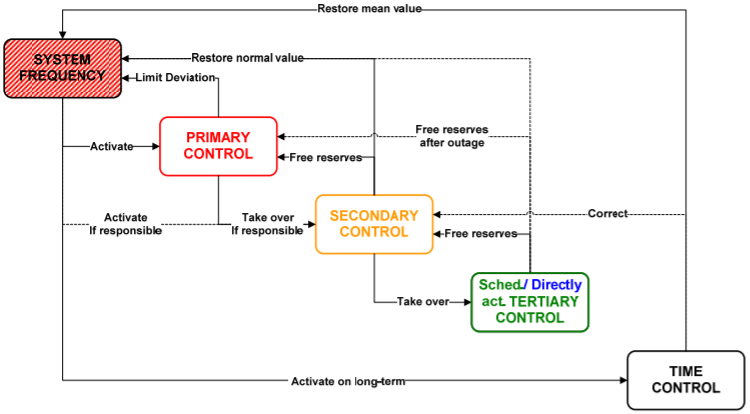
\includegraphics[width=0.9\textwidth]{figurer/Frekvenskontrol}
	\caption{Skematisk overblik over aktiveringen af kontrolreserver til frekvensregulering}
	\label{fig:Frekvenskontrol}
\end{figure}

ENTSO-E Policy 1 nedsætter også nogle krav til reservekapaciteten i det centraleuropæiske elnet. Vigtige krav er at den primære kontrol skal aktiveres ved frekvensafvigelser på $\pm$20mHz og den skal være fuldt ud aktiveret ved afvigelser på $\pm$200mHz. Størrelsen af den primære reserve bliver fastsat årligt og er på 3000MW. Den primære reserve er normeret fordelt på kraftværker i hele det centraleuropæiske elnet.

Den sekundære kontrol implementeres som en Load Frequency Control (LFC) struktur som vist på figur \ref{fig:sekundaerkontrol}. 

\begin{figure}[H]
	\centering
	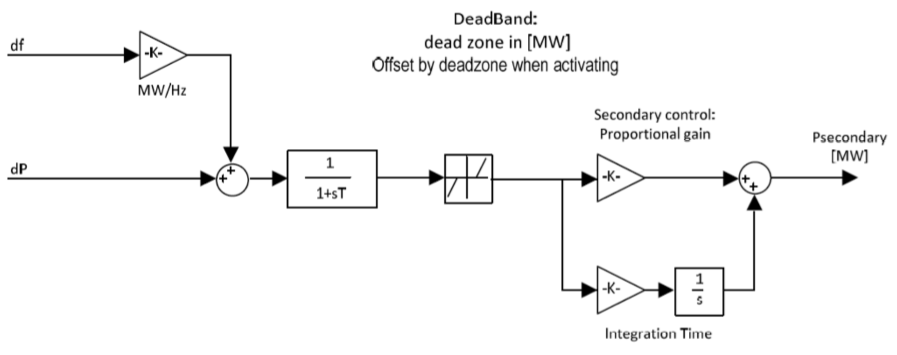
\includegraphics[width=0.9\textwidth]{figurer/Sekundaer_kontrol}
	\caption{LFC struktur}
	\label{fig:sekundaerkontrol}
\end{figure}

Ændringen i frekvens sammenholdes med ændringen i aktiv effekt gennem en K-faktor der er faktor der beregnes ud fra et område i systemets afvigelse fra systemfrekvensen i forhold til effektregulering pga. aktivering af den primære kontrol. Den samlede påkrævede effektregulering filtreres herefter og hvis afvigelsen i frekvens er udenfor et dødbåndsområde vil en PI regulator regulerer den generede effekt, sådan at systemfrekvensen igen kan opnåes.


VED IKKE OM DTE HER SKAL MED!
\textit{Et begreb der er relevant for et systems robusthed overfor forstyrrelser der vil påvirke frekvensen, er inerti. Dette skyldes at inerti har betydning for hvor hurtigt et system reagerer overfor ændringer. Et system med stor inerti vil have en længere responstid på forstyrrelse og frekvensændringen vil derfor sker langsommere. Dette er fordelagtigt, da det stiller mindre krav til hvor hurtigt den primære respons skal reagere. Typisk kommer inerti i elnettet fra synkrone maskiner, men da nyere vedvarende energikilder typisk er koblet til nettet gennem en frekvensomformer, bidrager de ikke med naturlig inerti. Der forskes derfor i hvordan kontrollen af frekvensomformere kan designes til at kunne generere "kunstig inerti". I dag anvendes der også synkron kondensere til at tilføre elnettet inerti.}


\section{Batterier som aktivt netelement}

Måden hvorpå batterier i elnettet kan bidrage til at stabilisere systemfrekvensen er at de både kan absorbere og genere effekt afhængigt af behovet og deres opladningstilstand. Dette kan give fordele i et elnet, hvor andelen er vedvarende energikilder er stor og derved har mindre reguleringsreserve i situationer med utilstrækkeligt vejr.

Her kan batterier fungere som både primær og sekundær reserve grundet den hurtige reguleringsmulighed der er i et rent elektrisk system. Et husstandsbatterier har en typisk kapacitet på 14kWh og kan levere 5kW nominelt og 7kW peak\footnote{TESLA}. Derfor vil enkelte husstandsbatterier ikke kunne bidrage særlig meget til balancering af produktion og forbrug, men en samling af mange husstandsbattier - en såkaldt aggrering vil kunne - vil kunne bidrage med betydelig effekt. Dette kombineret med muligheden for at oplade batterierne i perioder med mulighed for stor produktion fra grønne generationsenheder, så deres kapacitet er til rådighed i perioder med lav produktion fra grønne produktionsenheder kan tilføre den nødvendige fleksibilitet til elnettet for at kunne opretholde systemfrekvensen i en elnet med stor andel af vedvarende energikilder.

Placeringen og typen af batterierne forventes for frekvensstabiliteten at være ubetydelig, da den den generede effekt bare skal matche den absorberede for systemet for at opretholde den nominelle systemfrekvens. Det forventes heller ikke at have betydning for inertien i systemet hvor batterierne implementeres, da batterier er ikke roterende enheder og derfor ikke vil bidrage med naturlig inerti. En batteri inverter kunne muligvis designes til at kunne genere "kunstig inerti", men dette vil ikke blive undersøgt i dette projekt.


